\section{Istruzioni all'uso}

\subsection{Landing page}
All'avvio del prodotto verrà visualizzata la landing page, che presenta il logo dell'assistente virtuale e un messaggio di benvenuto. In questa fase, l'utente può scegliere di accedere al sistema.
\begin{figure}[h!]
    \centering
    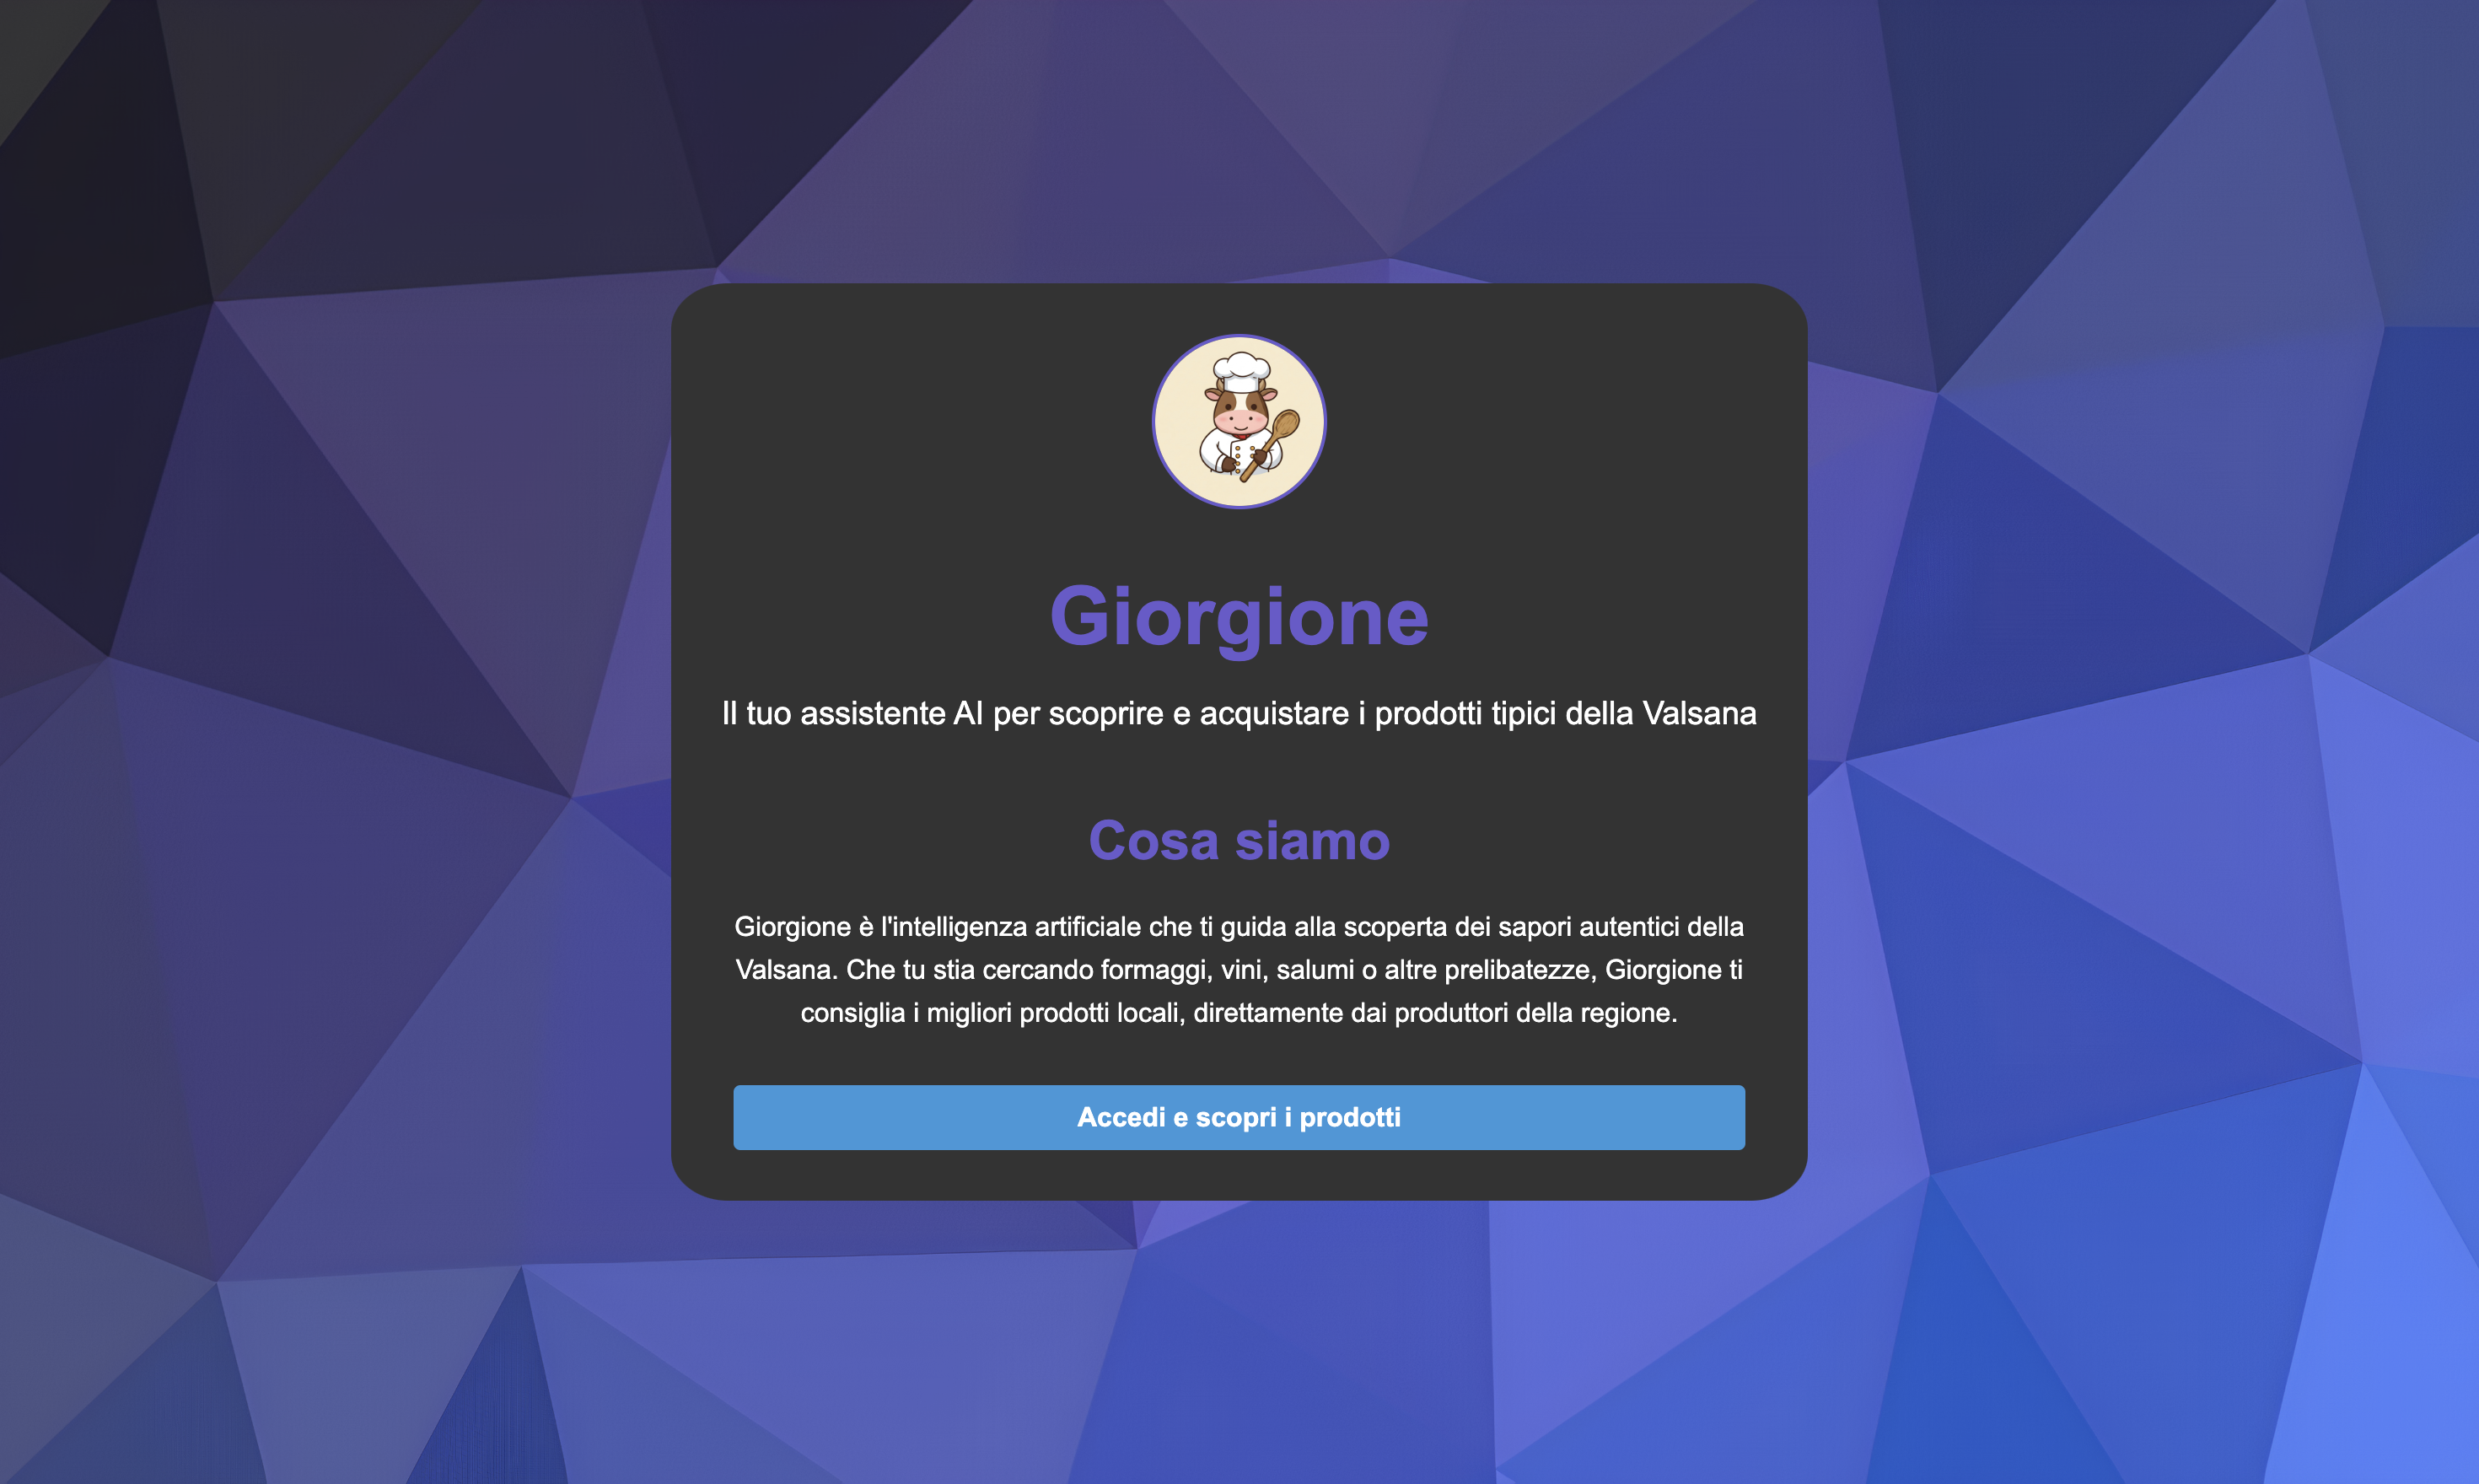
\includegraphics[width=0.8\textwidth]{./img/landingPage.png}
    \caption{Schermata della landing page}
\end{figure}

\subsection{Pagina di Accesso}
Cliccando sul bottone blu si passerà direttamente alla pagina di accesso, dove l'utente dovrà inserire le proprie credenziali (\textit{username} e \textit{password}) per autenticarsi.
\begin{figure}[h!]
    \centering
    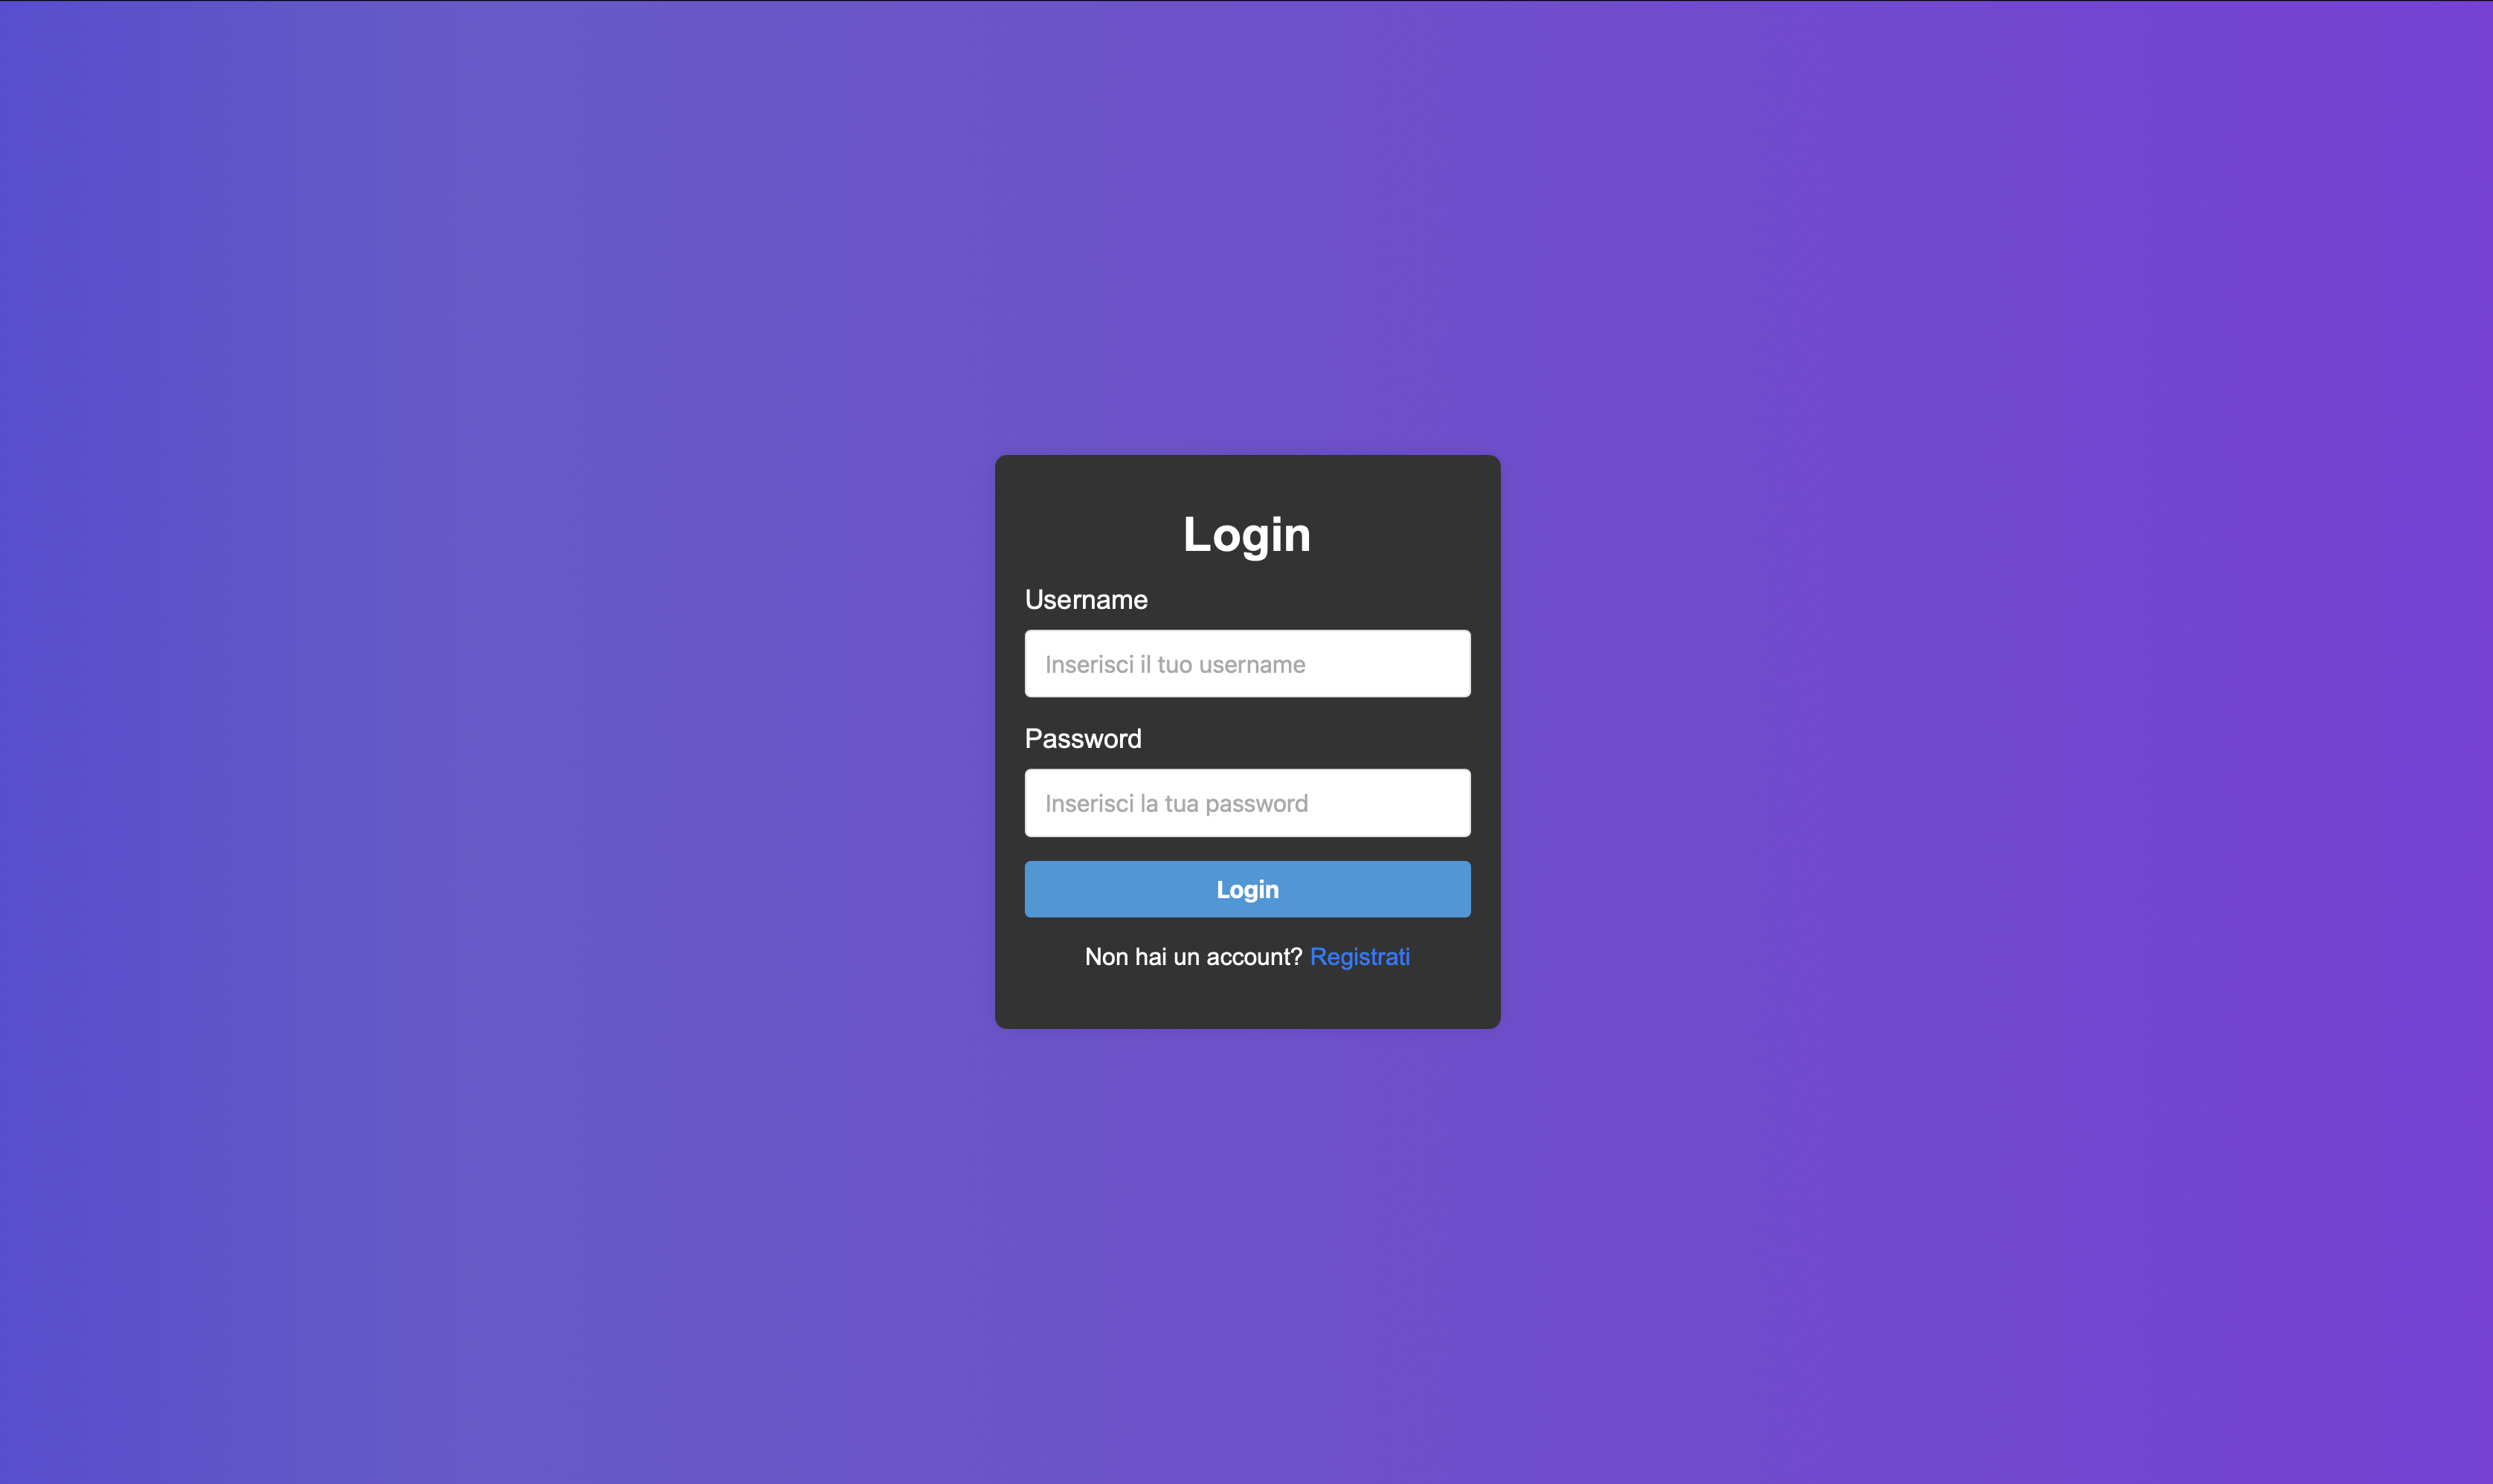
\includegraphics[width=0.8\textwidth]{./img/paginaAccesso.png}
    \caption{Schermata della pagina di accesso}
\end{figure}

\subsection{Pagina di Registrazione}
Nel caso in cui non si possieda un account, è possibile registrarsi dalla pagina di registrazione cliccando sul link presente nella pagina di autenticazione.
Qui l'utente dovrà inserire i campi obbligatori \{ \textit{username; password; email; nome; cognome} \} e volendo opzionalmente può inserire il numero di telefono.
\begin{figure}[h!]
    \centering
    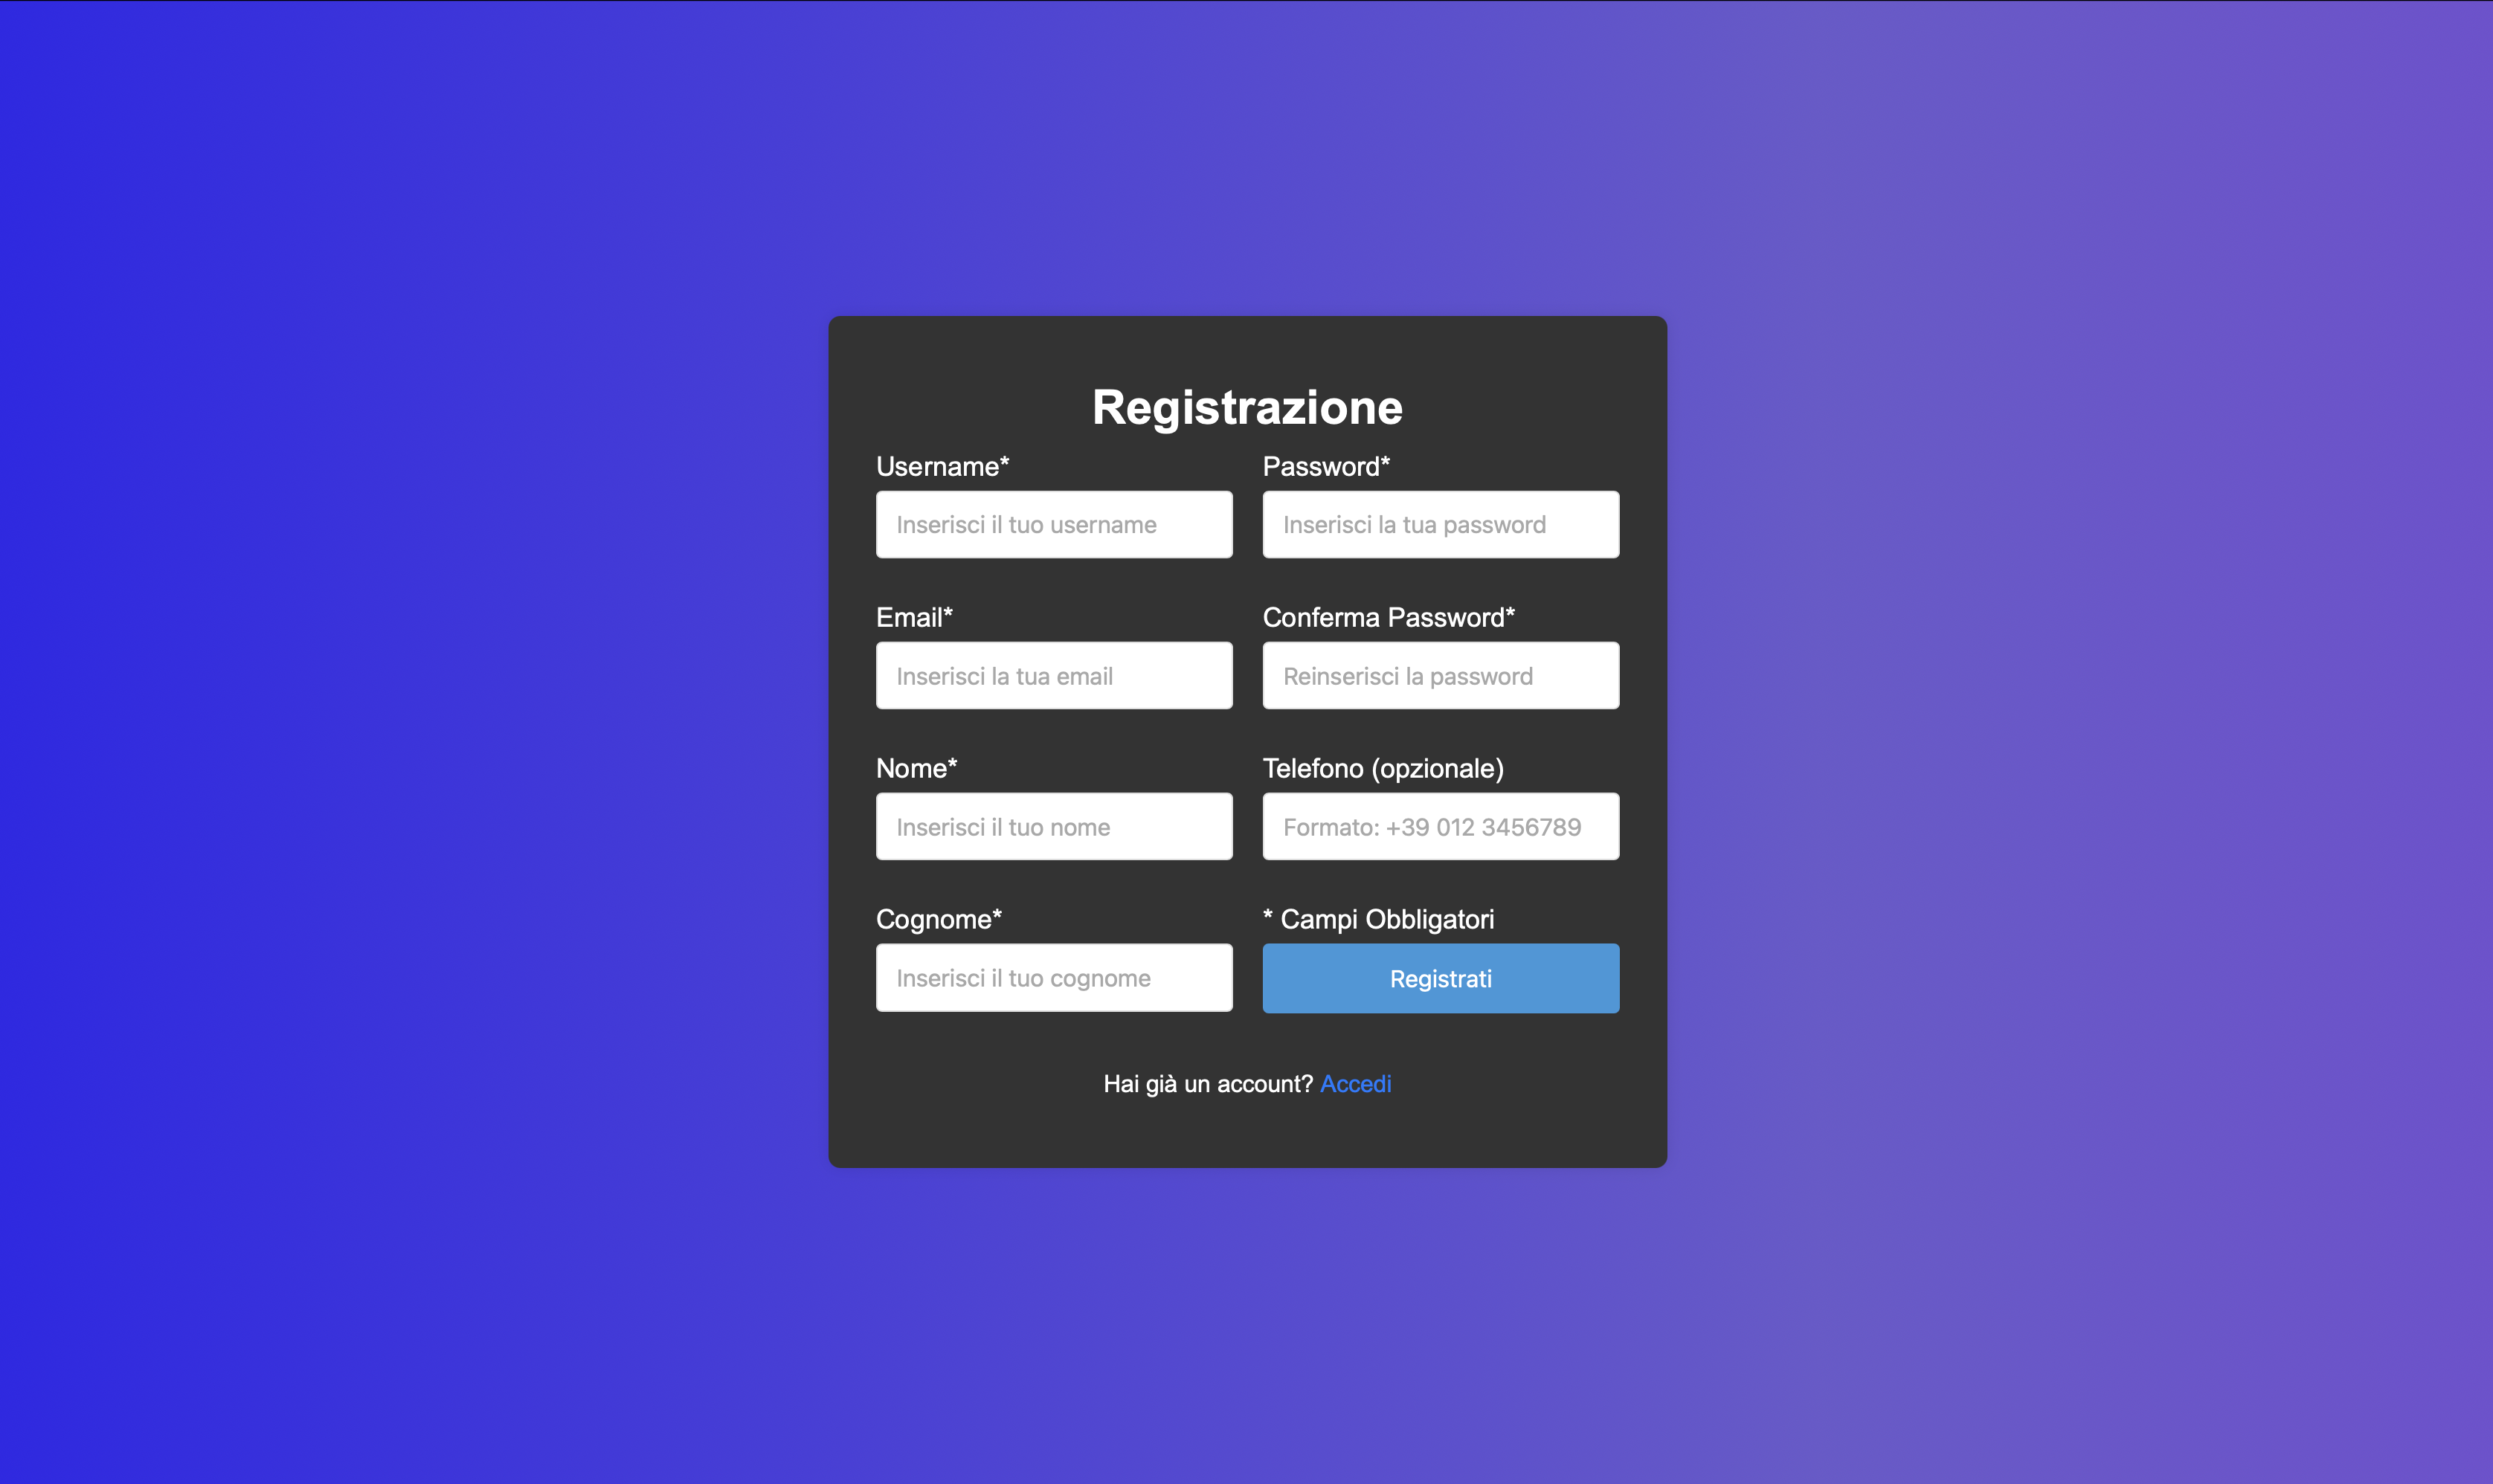
\includegraphics[width=0.8\textwidth]{./img/paginaRegistrazione.png}
    \caption{Schermata della pagina di registrazione}
\end{figure}

\subsection{Schermata iniziale}
Una volta effettuato l'accesso verremo accolti da questa Schermata iniziale composta da 3 elementi, una navbar superiore, una navbar laterale e il contenuto della pagina. Da qui è possibile iniziare una conversazione mettendo il titolo della conversazione e schiacciando il bottone: "inizia la conversazione".
\begin{figure}[h!]
    \centering
    \includegraphics[width=0.8\textwidth]{./img/paginaIniziale.png}
    \caption{Schermata della pagina di registrazione}
\end{figure}
